\secnumbersection{MARCO CONCEPTUAL}

\subsection{Base de Datos NoSQL}

\subsubsection{Definición}
Las bases de datos NoSQL (not only SQL) surgieron posterior a los sistemas de gestión de bases de datos relaciones (RDBMS, por sus siglas en inglés). Este término engloba todas las tecnologías de almacenamiento estructurada que no cumplen el esquema relacional \cite{del2013bases}.

El paradigma de bases de datos NoSQL surge a causa del cambio en el manejo de la infomación durante las últimas décadas. Hoy en día los volúmenes de infomación crecen a un ritmo sin precedentes, lo que ha complejizado su administración, es por este y otros motivos que la tecnlogía debe avanzar y crear sistemas que sean capaces de capturar estos cambios.

Existen dos razones principales que explican la necesidad de que surgan las bases de datos de NoSQL, estas son las siguientes \cite{romero2012utilidad}:

\begin{enumerate}
  \item \textbf{Tamaño y Cantidad de infomación:}  En el último tiempo el tamaño de los archivos ha crecido considerablemente, un ejemplo de esto han sido los archivos de video, el aumento de tamaño viene dado por la calidad del video. Las bases de datos relacionales tienen problemas de de escalabilidad, es decir, a medida que aumentan la cantidad de datos el desempeño disminuye.
  \item \textbf{Velocidad:} Es inaceptale que un usuario final tenga que esperar varios segundos en una consulta a una página web, esto se puede solucionar con sistemas distribuidos, pero las bases de datos relacionales no consideran esto puesto que fueron diseñadas y pensadas para sistemas pequeños, estructurados y centralizados.
\end{enumerate}

A pesar de que existen bases de datos NoSQL de varios tipos, todas ellas tienen las siguientes características en común \cite{romero2012utilidad}:

\begin{enumerate}
  \item \textbf{Escalabilidad Horizontal:} Facilidad de añadir, eliminar o realizar operaciones sin afectar el rendimiento.
  \item \textbf{Habilidad de distribución:} Replicar y distribuir los datos sobre distintos servidores.
  \item \textbf{Uso eficientes de recursos:} Aprovechar las nuevas tecnologías, como por ejemplo los discos sólidos.
  \item \textbf{Libertad de esquema:} No tiene esquema fijo, lo que facilita el modelamiento de datos y la integración con los lenguajes de programación.
  \item \textbf{Modelo de concurrencia débil:} No implementa ACID (Atomocidad, Consistencia, Aislamiento y Durabilidad), sin embargo, tiene algunas consideraciones para asegurar estos aspectos.
  \item \textbf{Consultas simples:} Consultas con menos operaciones y más naturales.
\end{enumerate}

\subsubsection{Bases de datos basadas en grafos}
Las bases de datos de grafos son un tipo de bases de datos NoSQL, que utiliza estructuras de grafos, compuesta por nodos, que son los objetos o entidades, y aristas, relaciones entre nodos, para representar y almacenar información. Los datos guardados en estas bases de datos son elementos interconectados con un número no determinado de relaciones entre ellos \cite{romero2012utilidad}.

Este tipo de base de datos se puede escalar de forma más natural a conjuntos de datos de mayor tamaño y son adecuadas para ambientes con esquemas de datos cambiantes y en estructuras de datos complejas. Las áreas de aplicación de este modelo son aquellas sobre las cuales la información sobre interconectividad o la topología de los datos es más o igual de importante que los datos en sí \cite{angles2008survey}. Esta es su principal motivación y característica, un ejemplo claro en donde se puede aplicar este tipo de base de datos son las redes sociales.

\begin{figure}[h]
\centering
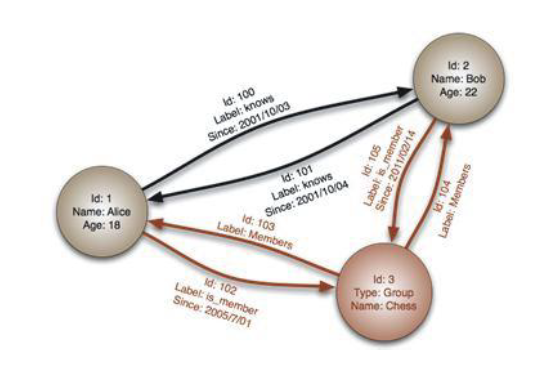
\includegraphics[width=0.5\textwidth]{ejemplo_grafo}
\caption{\label{fig:ejemplo_grafo} Representación de elementos en una base de datos de grafos.} Fuente: \cite{del2013bases}.
\end{figure}

\subsection{$k$-Anonymity}

La k-Anonimidad o \textit{k-Anonymity} esta basada en que es necesario producir datos anónimos, enfrentando dos problemas, el no revelar dicha información puede disminuir la necesidad de los datos y no proporcionar la protección adecuada puede ser perjudicial \cite{sweeney2002k}.

El ataque más común que intenta prevenir es la reidentificación mediante enlace, esto es emparejar o hacer \textit{matching} mediante atributos compartidos entre dos o más conjuntos de datos. Por ejemplo un conjunto tiene los datos médicos de las personas y otro contiene los datos electorales, ambos tienen atributos con sexo, fecha de nacimiento y código postal, al unir ambos conjuntos por sus atributos comunes, se puede revelar información importante acerca de las personas.

\begin{figure}[h]
\centering
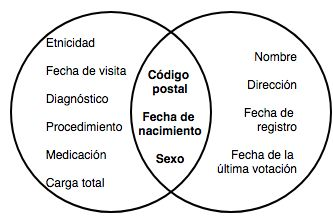
\includegraphics[width=0.4\textwidth]{ejemplo_matching}
\caption{\label{fig:linking_data} Reidentificar datos por enlace.} Fuente: \cite{sweeney2002k}.
\end{figure}

El término \textit{dato} se refiere a información específica de la persona que es conceptualmente organizada  como una tabla. Cada fila se denomina \textit{tupla} y cada columna se denomina \textit{atributo}, esta denota un campo o categoría de información con un conjuto de valores posibles. Al observar una tabla cada fila es una $n$-tupla de valores $<d_{1}, d_{2}, ..., d_{n}>$, donde $n$ es el número de columas. Este método asume que cada fila es una persona, no existiendo valores duplicados, con la finalidad de simplificar la explicación sin perder generalidad \cite{sweeney2002k}.

Utilizando el ejmplo de reidentificación por enlace (Figura \ref{fig:linking_data}), hay atributos como nombre, dirección y número de teléfono que son identificadores explícitos, estos facilitan que los conjuntos de datos se puedan vincular, pero existen otros atributos donde la combinación entre ellos también hace posible identificar a la persona, estos son llamados \textit{cuasi-identificador}, como por ejemplo la combinación entre sexo, fecha de nacimiento y código postal.

Determinar la cantidad de individuos que pueden ser identificados cuando se publican datos requiere de combinar los datos liberados con los externos y analizar los posibles ataques. Quien divulga los datos puede suponer los atributos que constituyen un  cuasi-identificador, pero no los valores que estos contienen en los datos externos, por lo tanto para protegerlos deben cumplir con la condición de $k$-Anonimato \cite{sweeney2002k}.

\begin{definicion}[$k$-Anonimidad]
Sea RT($A_{1}, A_{2}, ..., A_{n}$) un tabla y $QI_{RT}$ los cuasi-identificadores asociados a la tabla. Se dice que RT satisface la condición de $k$-Anonymity si y solo si cada valor de RT[$QI_{RT}$] aparece a lo menos $k$ veces en RT[$QI_{RT}$].
\end{definicion}

\begin{figure}[h]
    \centering
    \begin{tabular}{|c|c|c|c|c|c|}
        \hline
        & Raza & Año & Género & Código postal & Problema \\
        \hline
        $t_{1}$ & Negro & 1965 & m & 0214* & Corta respiración \\
        \hline
        $t_{2}$ & Negro & 1965 & m & 0214* & Dolor de pecho \\
        \hline
        $t_{3}$ & Negro & 1965 & f & 0213* & Hipertensión \\
        \hline
        $t_{4}$ & Negro & 1965 & f & 0213* & Hipertensión \\
        \hline
        $t_{5}$ & Negro & 1964 & f & 0213* & Obesidad \\
        \hline
        $t_{6}$ & Negro & 1964 & f & 0213* & Dolor de pecho \\
        \hline
        $t_{7}$ & Blanco & 1964 & m & 0213* & Dolor de pecho \\
        \hline
        $t_{8}$ & Blanco & 1964 & m & 0213* & Obesidad \\
        \hline
        $t_{9}$ & Blanco & 1964 & m & 0213* & Corta respiración \\
        \hline
        $t_{10}$ & Blanco & 1967 & m & 0213* & Dolor de pecho \\
        \hline
        $t_{11}$ & Blanco & 1967 & m & 0213* & Dolor de pecho \\
        \hline
    \end{tabular}
    \caption{\label{table:original} Ejemplo de $k$-Anonymity, donde $k$=2 y QI = $\lbrace$Raza, Año, género y código postal$\rbrace$} Fuente: \cite{sweeney2002k}.
\end{figure}

Para cada tupla de la tabla los valores de los cuasi-identificadores aparecen a lo menos dos veces en la tabla, por lo tanto satisface la condición de $k$-Anonimidad. Además cada valor de un cuasi-identificador aparece a lo menos dos veces.

Esta propiedad no garantiza que los individuos no puedan ser identificados dado que pueden existir otros ataques que revelen las identidades de las personas. Sin embargo este método protege los datos de una vinculación directa de ellos con fuentes externas y es una solución al problema de reindentificación por enlace (Figura \ref{fig:linking_data}).

\subsection{$\ell$-Diversity}
El método anterior si bien soluciona el problema de identificación por enlace, no resulve otros ataques y esto es porque no considera los atributos \textit{sensibles}, es decir, aquellos que no deben ser revelados al adversario \cite{machanavajjhala2006ell}.

\textbf{Ataque por Homogeneidad}: Se tiene la tabla descrita en la Figura \ref{fig:ataques}, en el último grupo como el valor de su atributo sensible es el mismo, si alguien conoce los datos de los cuasi-identificadores podria concluir que todos los que pertenecen a ese grupo tienen cáncer sin que esto sea correcto.

\begin{figure}[H]
    \centering
    \begin{tabular}{|c||c|c|c|c|}
        \hline
        & \multicolumn{3}{|c|}{\textit{Atributos no sensibles}} & \textit{Atributos sensibles} \\
        \hline
        & ZIP & Edad & Nacionalidad & Condición \\
        \hline
        1 & 130** & $<$ 30 & * & Enfermedad al corazón \\
        2 & 130** & $<$ 30 & * & Enfermedad al corazón \\
        3 & 130** & $<$ 30 & * & Infección viral \\
        4 & 130** & $<$ 30 & * & Infección viral \\
        \hline
        5 & 1485* & $\geq$ 40 & * & Cáncer \\
        6 & 1485* & $\geq$ 40 & * & Enfermedad al corazón \\
        7 & 1485* & $\geq$ 40 & * & Infección viral \\
        8 & 1485* & $\geq$ 40 & * & Infección viral \\
        \hline
        9 & 130** & 3* & * & Cáncer \\
        10 & 130** & 3* & * & Cáncer \\
        11 & 130** & 3* & * & Cáncer \\
        12 & 130** & 3* & * & Cáncer \\
        \hline
    \end{tabular}
    \caption{\label{fig:ataques}Tabla 4-Anonimidad con datos de pacientes internos en un hospital} Fuente: \cite{machanavajjhala2006ell}.
\end{figure}

\textbf{Ataque por conocimiento de fondo}: Utilizando la tabla de la Figura  \ref{fig:ataques}, si se tiene el conocimiento de que la probabilidad de que un grupo de personas sufra cierta enfermedad es bajo, por ejemplo lo que pasa en el primer grupo de la tabla donde solo hay dos valores posibles, entonces se concluye que el individuo padece de la enfermedad contraria.

Ambos ataques suceden porque \textit{k-Anonymity} crea grupos sin fijarse en la diversidad de valores que tienen los atributos sensibles dentro de cada uno, esto puede provocar que se revele información que sea perjudicial para los individuos.

Para solucionar el problema de privacidad se publica un tabla $T^{*}$,tabla generalizada y/o anonimizada de $T$, y dado el conocimiento del adversario esta tabla puede filtrar información de dos maneras: \textit{revelación positiva} y \textit{revelación negativa} \cite{machanavajjhala2006ell}.

\begin{definicion}[Revelación Positiva]
  Es aquella donde el adversario puede identificar, con alta probabilidad, el valor correcto del atributo sensible.
\end{definicion}

\begin{definicion}[Revelación Negativa]
  Es cuando el adversario puede eliminar correctamente algunos valores posible del atributo sensible, esto también con alta probabilidad.
\end{definicion}

Por eso motivos la tabla publicada $T^*$ debe entregar poca información adicional al adversario, es decir, no debe haber una gran diferencia entre lo que él conoce antes y después de publicar la tabla.

Para entender $\ell$-Diversity se considera un escenario ideal en el cual si dos objetos tienen un atributo no sensible ``similar'' entonces sus atributos sensibles también tienen un compartamiento probabilístico similar. En base a esto se define un \textit{q*-block} que es un conjunto de tuplas en $T^*$ cuyos valores de atributos no sensibles son generalizados en $q^*$, es necesario asegurar que para cada \textit{q*-block} los $\ell$ valores más frecuentes tengan la misma frecuencia, esto es la escencia de $\ell$-Diversity. Por lo tanto cumpliendo esto y realizando una buena partición de los datos, se puede evitar el ataque por conocimiento y las inferencias que se pueden hacer desde la tabla \cite{machanavajjhala2006ell}.

\begin{definicion}[Principio de $\ell$-Diversity]
  Un \textit{q*-block} es $\ell$-diverso si contiene a lo menos $\ell$ valores bien representados para el atributo sensible $S$. Una tabla es $\ell$-diverso is cada \textit{q*-block} es $\ell$-diverso.
\end{definicion}

Utilizando la tabla de la figura \ref{fig:ataques}, se aplica $\ell$-Diversity para solucionar el problema que tenia por homogeneidad del último grupo y se reordenan las tuplas generando la tabla descrita en la figura \ref{fig:l-divesity_ejemplo}.

\begin{figure}[H]
    \centering
    \begin{tabular}{|c||c|c|c|c|}
        \hline
        & \multicolumn{3}{|c|}{\textit{Atributos no sensibles}} & \textit{Atributos sensibles} \\
        \hline
        & ZIP & Edad & Nacionalidad & Condición \\
        \hline
        1 & 1305* & $<$ 40 & * & Enfermedad al corazón \\
        4 & 1305* & $<$ 40 & * & Infección viral \\
        9 & 1305* & $<$ 40 & * & Cáncer \\
        10 & 1305* & $<$ 40 & * & Cáncer \\
        \hline
        5 & 1485* & $\geq$ 40 & * & Cáncer \\
        6 & 1485* & $\geq$ 40 & * & Enfermedad al corazón \\
        7 & 1485* & $\geq$ 40 & * & Infección viral \\
        8 & 1485* & $\geq$ 40 & * & Infección viral \\
        \hline
        2 & 1306* & 3* & * & Enfermedad al corazón \\
        3 & 1306* & 3* & * & Infección viral \\
        11 & 1306* & 3* & * & Cáncer \\
        12 & 1306* & 3* & * & Cáncer \\
        \hline
    \end{tabular}
    \caption{\label{fig:l-divesity_ejemplo}Tabla 3-Diversa con datos de pacientes internos en un hospital} Fuente: \cite{machanavajjhala2006ell}.
\end{figure}

\subsection{Privacidad Diferencial}
Este método es estudiado y utilizado en bases de datos estadísticas, en donde el objetivo para preservar la privacidad es permitir que el usuario aprenda las propiedades de la población como un todo mientras se protege la privacidad del individuo, por lo tanto el acceder a una base de datos no debe permitir que el adversario aprenda algo sobre un individuo que no podria ser aprendido sin acceso \cite{dwork2011differential}.

Para resolver el problema planteado, se debe pasar de garantías absolutas a relativas, es decir, cualquier revelación será igual de probable sin importar que un individuo este o no presente en la base de datos. Para esto existen dos configuraciones posibles la interactiva y la no interactiva. En la primera, el \textit{curator}, se encuentra entre los usuarios y la base de datos, él puede modificar las consultas y/o respuestas de estas para proteger la privicidad de los participantes, los datos no pueden ser destruidos y el \textit{curator} debe permanecer presente durante toda la vida de la base de datos. En la configuración no interactiva el \textit{curator} calcula y publica algunas estadísticas y lo datos no se continúan utilizando \cite{dwork2008differential}.

Privacidad diferencial garantiza que la eliminación o adición de un único elemento a la base de datos no afecte el resultado de cualquier análisis.

\begin{definicion}
  Una función aleatorizada $K$ otorga $\epsilon$-privacidad diferencial si para todos los conjutos de datos $D_1$ y $D_2$, que difieren a lo más en un elemento, y para todo $S \subseteq Range(K)$, se cumple lo siguiente
  \begin{equation}
    Pr[K(D_1) \in S] \leq \exp(\epsilon) \times Pr[K(D_2) \in S]
  \end{equation}
\end{definicion}

Cuando la consulta es una función $f$, y la base de datos es $X$, la \textit{respuesta verdadera} es $f(X)$. El mecanismo $K$ lo que hace es agregar ruido aleatorio apropiadamente a la \textit{respuesta verdadera} para generar la respuesta \cite{dwork2008differential}. La magnitud de este ruido se elige como una función del cambio más grande que un único participante podría tener en el resultado de la función, se refiere a esta cantidad con la sensibilidad de la función \cite{dwork2011differential}.

\begin{definicion}
  Para $f$: $D \to R^d$, la L1-sensibilidad de $f$ es:
  \begin{equation}
    \begin{split}
      \Delta f & = \max_{D_1, D_2} || f(D_1) - f(D_2) ||_1 \\
              & = \max_{D_1, D_2} \sum_{i=1}^{d} |f(D_1)_i - f{D_2}_i|
     \end{split}
  \end{equation}
\end{definicion}

La sensibilidad de esta función da un límite superior sobre cuanto debemos perturbar su resultado para preservar la privacidad \cite{dwork2014algorithmic}. En particular cuando $d = 1$, la sensibilidad de $f$ es la diferencia máxima en los valores que esta función puede tomar en un par de bases de datos que difieren en una sola fila. Para muchos tipos de consultas $\Delta f$ será bastante pequeño, en especial las consultas de conteos simples, por ejemplo ¿Cuántas filas cumple la propiedad P? tiene $\Delta f = 1$. Las diferentes técnicas de privacidad diferencial funcionan mejor cuando tienen un valor de sensibilidad bajo. Notar que la sensibilidad es una valor solo de la función y no de la bases de datos \cite{dwork2008differential}.

Actualmente dos mecanismos básicos son usados para garantizar privacidad diferencial, estos son el mecanismo de Laplace y el mecanismo exponencial.

\subsubsection{Mecanismo de Laplace}

Para entender este mecanismo se debe conocer la distribución del Laplace.

\begin{definicion}
  La distribución de Laplace, centrada en 0 y con escala en $b$, tiene como función de densidad de probabilidad lo siguiente:
  \begin{equation}
    Lap(x|b) = \frac{1}{2b} \exp\left(- \frac{|x|}{b}\right)
  \end{equation}
\end{definicion}

Se denota $Lap(b)$ cuando se habla de la distribución de Laplace con escala en b. Cabe destacar que esta es una version simétrica de la distribución exponencial \cite{dwork2014algorithmic}.

Este mecanismo lo que hace es calcular $f$, y perturbar cada coordenada con ruido extraido de la distribución de Laplace. La escala del ruido es calibrada por la sensibilidad de $f$ dividido por $\epsilon$ \cite{dwork2014algorithmic}.

\begin{definicion}
    Dada cualquier función $f : N^{|\mathcal{X}|} \to R^k$, el mecanismo de Laplace es definido como:
    \begin{equation}
      \begin{split}
        \mathcal{M}_L(x, f(·), \epsilon) & = f(x) + (Y_1, ..., Y_k) \\
        \mathcal{M}(D) & = f(D) + Lap\left( \frac{\Delta f}{\epsilon}\right)
       \end{split}
    \end{equation}
    Donde $Y_i$ son variables aleatorias extraidas de $Lap(\Delta f/\epsilon)$
\end{definicion}

Este mecanismo tiene excelente precisión con consultas insensibles, es decir, de valor de sensibilidad bajo. En particular el ruido necesario para asegurar privacidad diferencial depende solo de la sensibilidad de la función y del parámetro $\epsilon$. Ambos son independientes de la base de datos y del número de filas que esta contenga. Por lo tanto, si la base de datos es muy grande los errores para las consultas típicas son relativamente pequeños \cite{dwork2008differential}.

\subsubsection{Mecanismo Exponencial}

Diseñado para situaciones en la que se requiere encontrar la mejor respuesta, pero agregar ruido directamente puede destruir por completo  su valor. El mecanismo exponencial es el componente natural para responder consultas con utilidades arbitrarias y un rango arbitrario no numérico, al tiempo en que se preseva privacidad diferencial. Dado un rango arbitrario $\mathcal{R}$, el mecanismo exponencial es definido con respecto a alguna función de utilidad $u: N^{|\mathcal{X}|} \times \mathcal{R} \to R$ que convierte los pares de bases de datos y/o salidas en puntajes de utilidad. Intuitivamente para una base de datos $x$, el usuario va a preferir que el mecanismo genere un elemento de $\mathcal{R}$ con el máximo puntaje de utilidad posible \cite{dwork2014algorithmic}.

\begin{definicion}
  Sensibilidad de $u$:
  \begin{equation}
    \Delta u = \max_{r \in \mathcal{R}} \left( \max_{x,y:||x - y||_1 < 1} | u(x,r) - u(y,r)| \right)
  \end{equation}
\end{definicion}

La intuición detrás de este mecanismo es generar cada posible $r \in \mathcal{R}$ con probabilidad proporcional a $\exp(\epsilon u(x,r)/\Delta u)$, pero esto pasa por alto algunos efectos de normalización que ocurren cuando una persona es añadida a la base de datos y puede causar que las utilidades de algunos elementos $r$ aumenten o disminuyan \cite{dwork2014algorithmic}. Por lo tanto el mecanismo exponencial debe considerar los cambios en términos de normalización.

\begin{definicion}
  El mecanismo exponencial $\mathcal{M}_E (x,u,\mathcal{R})$ selecciona y genera un elemento $r \in \mathcal{R}$ con probabilidad proporcional a $\exp\left(\frac{\epsilon u(x,r)}{2\Delta u}\right)$
  \begin{equation}
    \mathcal{M}(x) = \left( \textup{return } r \propto \exp\left( \frac{\epsilon u(x,r)}{2\Delta u} \right) \right)
  \end{equation}
\end{definicion}

Este mecanismo es utilizado para consultas no numéricas donde la función de utilidad busca evaluar la calidad de la respuesta. La definición de una función de utilidad depende de la aplicación, por lo tanto diferentes aplicaciones conducen a varias funciones de utilidad \cite{zhu2017differentially}.


% Se debe describir la base conceptual o fundamentos en los que se basa tu memoria, es decir, todos los conceptos técnicos, metodologías, herramientas, etc. que están involucradas en la solución propuesta. En el fondo esta parte permite precisar y delimitar el problema, estableciendo definiciones para unificar conceptos y lenguaje y fijar relaciones con otros trabajos o soluciones encontradas por otros al mismo problema evitando así plagios o repetir errores ya conocidos o abordados por otros.
%
% En esta parte es importante relacionar estos conceptos con la memoria y es fundamental utilizar referencias bibliográficas (o de la web) recientes, por ejemplo \cite{gettelfinger2004will}.
